%%%%%%%%%%%%%%%%%%%%%%%%%%%%%%%%%%%%%%
% LaTeX poster template
% Created by Nathaniel Johnston
% August 2009
% http://www.nathanieljohnston.com/2009/08/latex-poster-template/
%%%%%%%%%%%%%%%%%%%%%%%%%%%%%%%%%%%%%%

\documentclass[final]{beamer}
\usepackage[scale=0.8]{beamerposter}
\usepackage{graphicx}			% allows us to import images
%\beamertemplategridbackground[1in]

\usepackage{bm}
\usepackage{tikz}
\usepackage{times}

\usetikzlibrary{trees,shadows,fit,positioning,calc}


%-----------------------------------------------------------
% Define the column width and poster size
% To set effective sepwid, onecolwid and twocolwid values, first choose how many columns you want and how much separation you want between columns
% The separation I chose is 0.024 and I want 4 columns
% Then set onecolwid to be (1-(4+1)*0.024)/4 = 0.22
% Set twocolwid to be 2*onecolwid + sepwid = 0.464
%-----------------------------------------------------------

\newlength{\sepwid}
\newlength{\onecolwid}

% A0 paper dimensions
\setlength{\paperwidth}{38.8in}
\setlength{\paperheight}{24.0in}

\setlength{\sepwid}{0.060\paperwidth}
\setlength{\onecolwid}{0.30\paperwidth}
\setlength{\topmargin}{-0.5in}
\usetheme{confposter}
%\usepackage{exscale}

%\input{preamble}


%-----------------------------------------------------------
% The next part fixes a problem with figure numbering. Thanks Nishan!
% When including a figure in your poster, be sure that the commands are typed in the following order:
% \begin{figure}
% \includegraphics[...]{...}
% \caption{...}
% \end{figure}
% That is, put the \caption after the \includegraphics
%-----------------------------------------------------------

\usecaptiontemplate{
\small
\structure{\insertcaptionname~\insertcaptionnumber:}
\insertcaption}

%-----------------------------------------------------------
% Define colours (see beamerthemeconfposter.sty to change these colour definitions)
%-----------------------------------------------------------

% \setbeamercolor{block title}{fg=ngreen,bg=white}
% \setbeamercolor{block body}{fg=black,bg=white}
% \setbeamercolor{block alerted title}{fg=white,bg=dblue!70}
% \setbeamercolor{block alerted body}{fg=black,bg=dblue!10}

%-----------------------------------------------------------
% Name and authors of poster/paper/research
%-----------------------------------------------------------

\title{Articulated Motion Models for Scene Understanding}
\author{Suren Kumar$^1$ \and Vikas Dhiman$^2$ \and Jason J Corso$^2$ \and Venkat N. Krovi$^1$}
\institute{$^1$University at Buffalo  \hspace{1in} $^2$University of Michigan}

%-----------------------------------------------------------
% Start the poster itself
%-----------------------------------------------------------

\begin{document}

\begin{frame}[t]
  \centering
  \begin{columns}[t]												% the [t] option aligns the column's content at the top
  %\begin{column}{\sepwid}\end{column}			% empty spacer column
  \hspace{-\sepwid}
    \begin{column}{\onecolwid}
      \begin{block}{Introduction}
        Imagine a robot moving in a typical living room environment which encounters indoor objects such as doors, drawers and chairs etc. We posit that in order for the robot to understand, map or interact with such objects, the robot needs to be able to understand the articulation. 

        \begin{figure}
          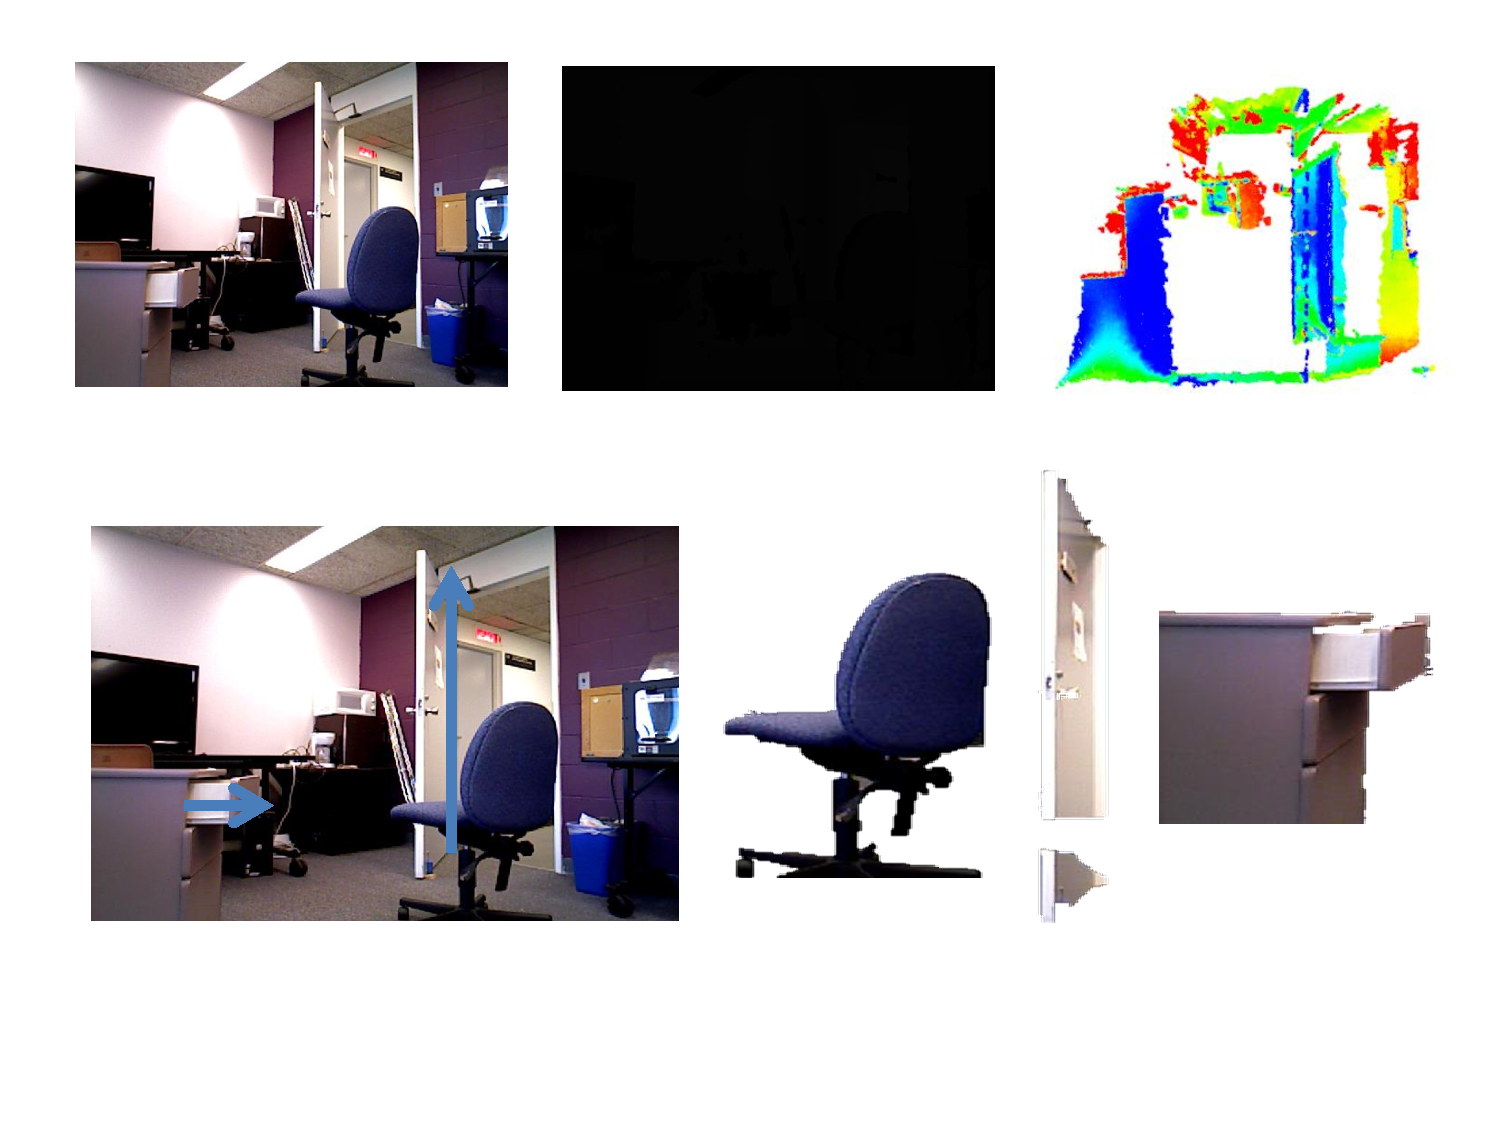
\includegraphics[width=\onecolwid,trim=0 1in 0 3in,clip]{media/parts_of_scenes}
          \caption{World is composed of rigid bodies. These rigid bodies are connected to each other by limited types of joints $\{C_j\}$, for example, static, prismatic etc
}
        \end{figure}
      \end{block}

      \begin{block}{Modeling}
        \begin{figure}
          \centering
          \newcommand{\imagewidth}{\onecolwid}
          \scalebox{2.0}{\tiny \begin{tikzpicture}
\tikzstyle{main}=[circle, minimum size = 10mm, thick, draw =black!80, node distance = 10mm]
\tikzstyle{connect}=[-latex, thick]
\tikzstyle{box}=[rectangle, draw=black!100]
\coordinate (org_1) at (0,0);
  \node[main] (x_k_1)[right=of org_1] {$x_{k-1}$ };
  \node[main] (x_k) [right=of x_k_1] { $x_{k}$ };
  \node[main] (x_k_2) [right=of x_k] {$x_{k+1}$};
\coordinate[right=of x_k_2] (end_1);

  \node[main, fill = black!20] (u_k_1)[above=of x_k_1.west] {$u_{k-1}$ };
\node[main, fill = black!20] (u_k)[above=of x_k.west] {$u_{k}$ };
\node[main, fill = black!20] (u_k_2)[above=of x_k_2.west] {$u_{k+1}$ };

\node[main, fill = black!20] (z_k_1)[below=of x_k_1.east] {$z_{k-1}$ };
\node[main, fill = black!20] (z_k)[below=of x_k.east] {$z_{k}$ };
\node[main, fill = black!20] (z_k_2)[below=of x_k_2.east] {$z_{k+1}$ };


\node[main] (m_k_1)[below=of z_k_1.west] {$m_{k-1}$ };
\coordinate [left=of m_k_1](org_2);
\node[main] (m_k)[below=of z_k.west] {$m_{k}$ };
\node[main] (m_k_2)[below=of z_k_2.west] {$m_{k+1}$ };
\coordinate [right=of m_k_2](end_2);

\node[main] (v_k_1)[below=of m_k_1.east] {$v_{k-1}$ };
\node[main] (v_k)[below=of m_k.east] {$v_{k}$ };
\node[main] (v_k_2)[below=of m_k_2.east] {$v_{k+1}$ };


  \path 
 (org_1) edge [connect] (x_k_1)
(x_k_1) edge [connect] (x_k)
(x_k) edge [connect] (x_k_2)
(x_k_2) edge [connect] (end_1)

(u_k_1) edge [connect] (x_k_1)
(u_k) edge [connect] (x_k)
(u_k_2) edge [connect] (x_k_2)

(x_k_1) edge [connect] (z_k_1)
(x_k) edge [connect] (z_k)
(x_k_2) edge [connect] (z_k_2)

(m_k_1) edge [connect] (z_k_1)
(m_k) edge [connect] (z_k)
(m_k_2) edge [connect] (z_k_2)


 (org_2) edge [connect] (m_k_1)
(m_k_1) edge [connect] (m_k)
(m_k) edge [connect] (m_k_2)
(m_k_2) edge [connect] (end_2)

(v_k_1) edge [connect] (m_k_1)
(v_k) edge [connect] (m_k)
(v_k_2) edge [connect] (m_k_2);
\end{tikzpicture}
}
          \caption{Graphical Model of the general SLAM problem. The known nodes are darker than the unknown nodes.
}
        \end{figure}

      \end{block}
      \begin{block}{Time Update}

        The time update models the evolution of state according to the motion model. To write equation concisely, let $A =\{ \mathbf{Z}_{0:k-1},\mathbf{U}_{0:k},\mathbf{V}_{0:k},x_0,m_0 \}$
        \begin{multline}
          P(x_k,m_k|A) = 
          % &\int \int P(x_k,x_{k-1},m_k,m_{k-1}|A) dx_{k-1} dm_{k-1} \nonumber \\
          % &\int \int P(x_k|x_{k-1},m_k,m_{k-1},A)P(x_{k-1},m_k,m_{k-1}|A) dx_{k-1}dm_{k-1} \nonumber \\
          % &\int \int P(x_k|x_{k-1},u_k)P(x_{k-1},m_k,m_{k-1}|A) dx_{k-1}dm_{k-1} \nonumber \\
          % &\int \int P(x_k|x_{k-1},u_k)P(m_k|x_{k-1},m_{k-1},A)P(x_{k-1},m_{k-1}|A)  dx_{k-1}dm_{k-1} \nonumber \\
          \int \int 
          \underbrace{P(x_k|x_{k-1},u_k)}_{\text{Robot motion}}
          \underbrace{P(m_k|m_{k-1},v_{k-1})}_{\text{World motion}}
          \underbrace{P(x_{k-1},m_{k-1}|A)}_{\text{Previous state}} dx_{k-1}dm_{k-1}
          \label{eq:time_update}
        \end{multline}

        \begin{itemize}
          \item
            Robot motion can be obtained from the kinematic/dynamic model 
          \item 
            World motion is approximated by finite order motion model
        \end{itemize}

      \end{block}
    \end{column}
  \hspace{-\sepwid}

  %\begin{column}{\sepwid}\end{column}			% empty spacer column

      
    \begin{column}{\onecolwid}
      \begin{block} {Measurement Update} Measurement update uses the Bayes formula to update the state of the estimation problem given a new observation $z_k$ at time step $k$. To write the equations concisely, let $B =\{ \mathbf{Z}_{0:k},\mathbf{U}_{0:k},\mathbf{V}_{0:k},x_0,m_0 \}$
        \begin{align}
          P(x_k,m_k|B) %&= \frac{P(z_k|x_k,m_k,A)P(x_k,m_k|A)}{P(z_k|A)} \nonumber\\
          &=\frac{P(z_k|x_k,m_k)P(x_k,m_k|A)}{P(z_k|A)}
          \label{eq:measurement_update}
        \end{align}

      \end{block}

      \begin{block}{Dynamic World Representation} 
        We assume a uniform prior $\mu_j(0) = P(C_j), \sum_{j=1}^{p}\mu_j(0) = 1$ over different motion models for each scene part. Note that, this prior can be modified appropriately by object detection such as doors are more likely to have revolute joints etc. 
        \begin{align*}
          & \mu_j(k) \equiv P(C_j|\mathbf{Z}_{0:k})  = 
          %\frac{P(z_k|\mathbf{Z}_{0:k-1}, C_j)P(C_j|\mathbf{Z}_{0:k-1})}{P(z_k|\mathbf{Z}_{0:k-1})} \nonumber \\
          %&\mu_j(k) = 
          \frac{P(z_k|\mathbf{Z}_{0:k-1}, C_j)\mu_j(k-1)}{\sum_{j=1}^{p} P(z_k|\mathbf{Z}_{0:k-1}, C_j)\mu_j(k-1) }
        \end{align*}
      \end{block}

      \begin{block}{Temporal Modeling}
        \begin{align}
          \begin{bmatrix}
            x^{1} \\
            x^{2} \\
            . \\
            .\\
            x^{n}
          \end{bmatrix} &= 
          \begin{bmatrix}
            0 & 1  & . & . & 0\\
            0 & 0  & . & . & 0\\
            0 & 0  & . & . & 0\\
            0& 0 & . & . & 1\\
            0 & 0  & . & . & 0\\
          \end{bmatrix}
          \begin{bmatrix}
            x \\
            x^{1} \\
            . \\
            .\\
            x^{n-1}
          \end{bmatrix}
          +\begin{bmatrix}
            0 \\
            0 \\
            .\\
            .\\
            1
          \end{bmatrix} 
          \eta\\
        y &=  \begin{bmatrix}
          1 &
          0 &
          .&
          .&
           0
          \end{bmatrix} 
        \begin{bmatrix} x \\ x^{1} \\ . \\ .\\ x^{n-1} \end{bmatrix} + \omega
        \end{align}
        where $x^{n}$ denotes $n^{th}$ order derivative of the state variable and $\eta$ and $\omega$ are process and observation noise. 
      \end{block}

      \begin{block}{Experiments and Results}
        \begin{figure}
          \newlength{\imgwidth}
          \setlength{\imgwidth}{\textwidth}
          \centering
          \tikzset{/tikz/x=0.08\linewidth}
          \tikzset{/tikz/y=0.08\linewidth}
           \begin{tikzpicture}[imgstyle/.style={draw,thick,anchor=south west,inner sep=1pt}]
 %\path[use as bounding box, draw] (0,-1) rectangle (\imgwidth, 0.34\imgwidth);
\node[imgstyle] (img1) at (0,0) {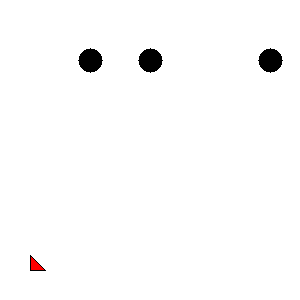
\includegraphics[width=0.32\imgwidth]{media/frame0000.png}};
\node[imgstyle] (img2) at (0.333\imgwidth,0) {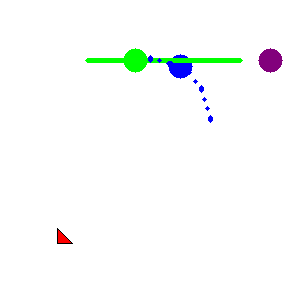
\includegraphics[width=0.32\imgwidth]
{media/frame0003.png}};
\node[imgstyle] (img3) at (0.666\imgwidth,0) {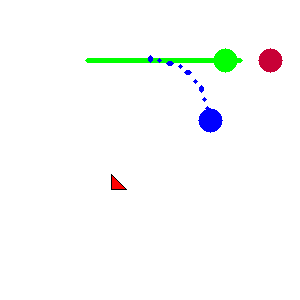
\includegraphics[width=0.32\imgwidth]{media/frame0009.png}};
\begin{scope}[x={(img1.south east)}, y={(img1.north west)}]
\node (r) at (0.3, 0.1) {Robot};
\node (lmks) at (0.7, 0.6) {Landmarks};
\end{scope}
\path ($(img1.south) + (-0.5, -0.5)$) node (ld) {Legend:};
\path 
(ld)
 ++ (1.8, 0) node [circle,fill=green] {} + (1, 0) node {Prismatic}
 ++ (3, 0) node [circle,fill=blue] {} + (1, 0) node {Revolute}
 ++ (3, 0) node [circle,fill=red] {} + (0.8, 0) node {Static}
;

 \end{tikzpicture}
%
          \caption{ Frames at different time intervals of our simulation.
      Color of a landmark at a particular frame is the weighted sum of colors
      assigned to each motion model. The weights used are the probability of the
    landmark following that particular motion model and estimated by our algorithm. We also show the predicted trajectory of a landmark according to the estimated motion model.}
          \label{fig:graphmodel}
        \end{figure}
      \end{block}

      
    \end{column}

  %\begin{column}{\sepwid}\end{column}			% empty spacer column

  \hspace{-\sepwid}
    \begin{column}{\onecolwid}

      \begin{block}{Temporal Model Simulation}
        \centering
          \begin{figure}
            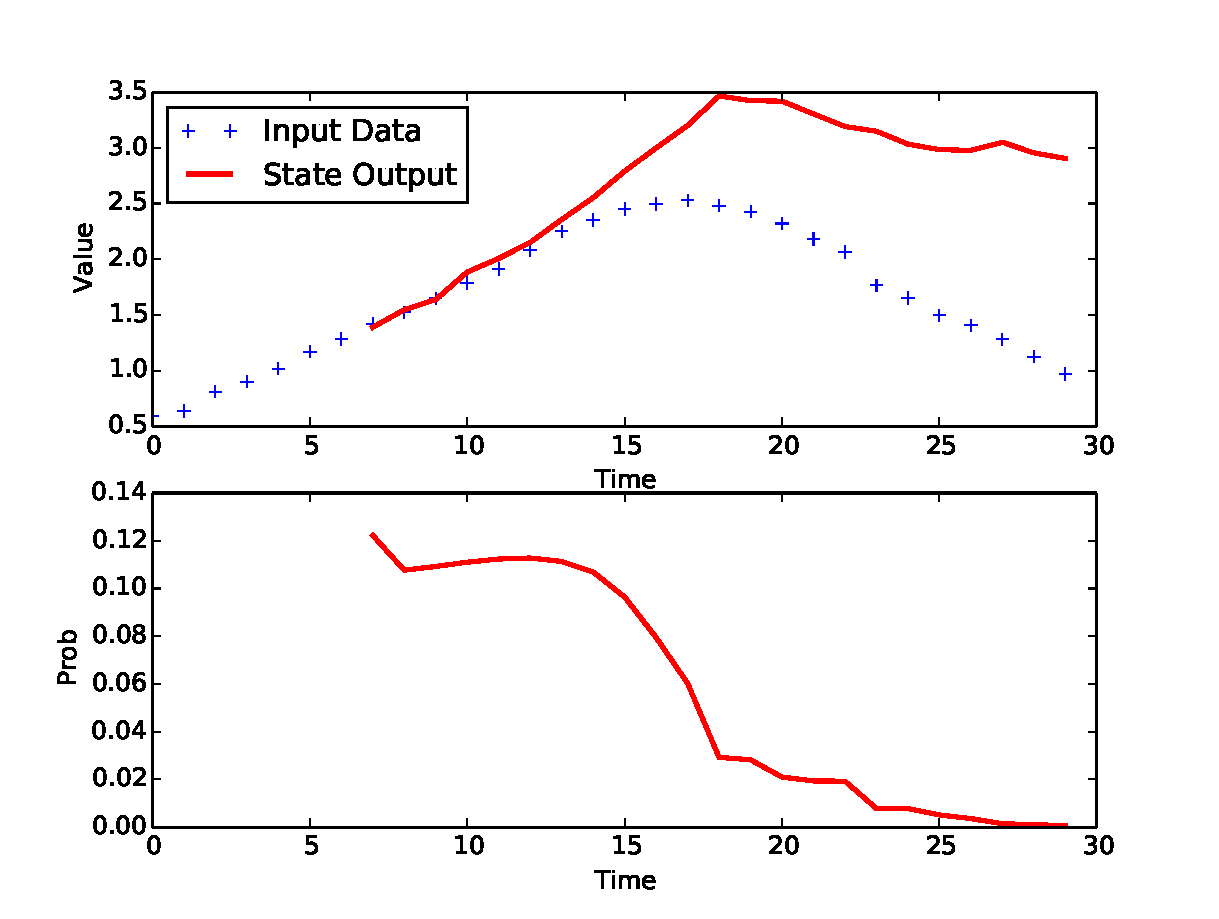
\includegraphics[width=1.0\onecolwid]{media/temporal_model.pdf}
            \caption{The ``Input Data'' is time varying parameter of the world
            motion, which is approximated by a first order motion model and
          it's trajectory is shown as ``State output''. The later plot show the
        probability of the motion model explaining the observed model. The
      probability decreases drastically after only a few frames.}
          \end{figure}
      \end{block}

      \begin{block}{Conclusion and Future Work}
        \begin{itemize}
          \item We use constraints in the physical world to model dynamic world
          \item Finite order motion models can explain any motion locally
          \item We need further real world experiments to prove the effectiveness of our model
        \end{itemize}
      \end{block}
      \begin{block}{References}
        \nocite{yaakov2001estimation}
        \nocite{cifuentes2012motion}
        \nocite{yan2006automatic}
        {\small
        \bibliographystyle{plain}
        \bibliography{../paper/cvpr_abstract/articulation_scene_understanding}
        }
      \end{block}
    \end{column}

  \begin{column}{\sepwid}\end{column}			% empty spacer column

  \end{columns}
\end{frame}
\end{document}

\setbeamercolor{block alerted title}{fg=black,bg=norange}	% frame color
\setbeamercolor{block alerted body}{fg=black,bg=white}		% body color
\begin{alertblock}{Alert Block Colours}
  You can similarly modify the colours for alert blocks (but try not to overdo it):\\
  \begin{semiverbatim}
  {\color{red}\\setbeamercolor}\{block title\}\newline \{fg=black,bg=norange\}
  \end{semiverbatim}
  \begin{semiverbatim}
  {\color{red}\\setbeamercolor}\{block  body\}\newline \{fg=black,bg=white\}
  \end{semiverbatim}
\end{alertblock}        
